\section{Pendahuluan}
\subsection{Latar Belakang}
Mikrokontroler adalah komputer mini dalam satu chip yang menggabungkan CPU, memori, dan periferal (GPIO, ADC, timer, antarmuka serial) sehingga dapat membaca kondisi lingkungan dan mengendalikan perangkat secara langsung. Komponen ini menjadi inti dari sistem tertanam yang ada pada perangkat sehari-hari, mulai dari peralatan rumah tangga, sensor IoT, hingga kontroler pada robot dan mesin industri. Karena itu, seorang insinyur komputer perlu memahami cara memprogram mikrokontroler, memilih platform yang tepat, dan menghubungkannya dengan dunia fisik.

Modul 1 ini memperkenalkan dua platform yang akan dipakai sepanjang praktikum, yaitu STM32 Blackpill (framework Arduino) dan ESP32 (framework ESP-IDF dan Arduino). Praktikan juga diperkenalkan pada tiga kemampuan dasar yang selalu muncul pada hampir semua sistem tertanam: membaca masukan digital dari tombol (pull-up dan pull-down), menangani gangguan sinyal pada tombol mekanik (debouncing), dan membaca besaran analog melalui ADC. Permasalahan yang ingin diselesaikan adalah bagaimana mikrokontroler dapat membaca masukan dari dunia nyata secara andal, yaitu tidak terbaca acak (floating), tidak terbaca ganda (bouncing), dan terbaca dengan resolusi yang sesuai (ADC), serta bagaimana lingkungan pengembangan disiapkan agar program dapat ditulis dan di-flash ke board. Pemahaman ini menjadi fondasi untuk modul-modul berikutnya, seperti sensor dan aktuator, komunikasi serial, interrupt dan multitasking, serta sistem kontrol.

\subsection{Dasar Teori}
\subsubsection{PlatformIO dan VSCode}
PlatformIO adalah ekosistem pengembangan embedded lintas platform yang berjalan sebagai ekstensi di Visual Studio Code. PlatformIO mendukung banyak board dan framework (Arduino, STM32Cube/HAL, ESP-IDF, dan lainnya) dalam satu antarmuka yang seragam. Struktur project-nya terdiri atas \texttt{platformio.ini} (konfigurasi board, framework, dan upload protocol), \texttt{src/} (kode program utama), \texttt{include/} (header), dan \texttt{lib/} (pustaka tambahan). Chip yang sama dapat diprogram dengan framework berbeda hanya dengan mengubah \texttt{platformio.ini}.

\subsubsection{STM32 Blackpill, ST-Link, dan Framework Arduino}
STM32 Blackpill adalah board berbasis mikrokontroler STM32F401CC (ARM Cortex-M4 dengan FPU, clock hingga 84 MHz, Flash 256 KB, RAM 64 KB). LED onboard berada pada pin PC13 (aktif LOW) dan tombol pengguna pada pin PA0. Board ini tidak memiliki programmer onboard, sehingga pada praktikum ini di-flash menggunakan ST-Link eksternal melalui protokol SWD (SWDIO, SWCLK, GND, dan 3,3 V). STM32 diprogram dengan framework Arduino (STM32duino) yang menyediakan fungsi seperti \texttt{pinMode()}, \texttt{digitalWrite()}, dan \texttt{delay()}, sementara di baliknya tetap memakai HAL dari STMicroelectronics.

\subsubsection{ESP32 dan Framework ESP-IDF}
ESP32 adalah mikrokontroler 32-bit dual-core dengan WiFi dan Bluetooth terintegrasi. Board DevKit-nya dilengkapi chip USB-to-Serial sehingga dapat diprogram langsung melalui kabel USB. ESP-IDF adalah framework resmi dan native dari Espressif yang dibangun di atas FreeRTOS, dengan titik masuk \texttt{app\_main()} dan pengaturan waktu memakai \texttt{vTaskDelay()}. Sebagai pembanding, framework Arduino memakai struktur \texttt{setup()} dan \texttt{loop()} dengan \texttt{delay()}, tingkat abstraksinya lebih tinggi, tetapi akses ke fitur RTOS lebih terbatas.

\subsubsection{Pull-up dan Pull-down Resistor}
Pin input yang tidak terhubung ke level tegangan apa pun berada dalam kondisi \emph{floating}, sehingga nilai yang terbaca tidak pasti akibat noise. Resistor pull-up menghubungkan pin ke VCC sehingga pin terbaca HIGH saat tombol tidak ditekan dan LOW saat tombol (yang dihubungkan ke GND) ditekan. Resistor pull-down menghubungkan pin ke GND sehingga pin terbaca LOW saat tombol tidak ditekan dan HIGH saat tombol (yang dihubungkan ke VCC) ditekan. Resistor ini dapat berupa komponen eksternal (umumnya 10 k$\Omega$) atau diaktifkan lewat firmware, yaitu \texttt{INPUT\_PULLUP} dan \texttt{INPUT\_PULLDOWN} pada ESP32. Pin input-only ESP32 (GPIO 34--39) tidak memiliki resistor pull internal.

\subsubsection{Debouncing}
Kontak mekanik pada tombol menghasilkan beberapa transisi HIGH--LOW dalam waktu sangat singkat akibat getaran saat kontak bersentuhan atau terlepas (\emph{bouncing}). Tanpa penanganan, satu kali penekanan dapat terbaca sebagai beberapa event. Debouncing memastikan hanya satu transisi valid yang diterima, misalnya dengan menunggu sinyal stabil selama 20--50 ms sebelum dianggap sah.

\subsubsection{ADC}
Selain digital output dan digital input, GPIO dapat dipakai sebagai analog input melalui ADC (\emph{Analog-to-Digital Converter}) yang mengubah tegangan kontinu menjadi nilai digital. ESP32 memiliki ADC internal dengan resolusi default 12-bit (nilai 0--4095) dan rentang tegangan sekitar 0--3,3 V, diakses dengan \texttt{analogRead()} pada framework Arduino. Pin ADC1 (misalnya GPIO 32--39) lebih disarankan daripada ADC2 karena ADC2 memiliki keterbatasan saat WiFi aktif.

Seluruh teori di atas mengacu pada Modul 1 Praktikum Sistem Tertanam.

%===========================================================%
\section{Tugas Pendahuluan}
Berikut jawaban tugas pendahuluan beserta penjelasannya.
\begin{enumerate}
	\item Jelaskan perbedaan mendasar antara framework Arduino dan ESP-IDF dalam memprogram mikrokontroler, termasuk kelebihan dan kekurangan masing-masing.

	\textbf{Jawaban:} Arduino adalah framework dengan tingkat abstraksi tinggi. Program disusun dari \texttt{setup()} yang berjalan sekali dan \texttt{loop()} yang berulang, dengan fungsi sederhana seperti \texttt{pinMode()}, \texttt{digitalWrite()}, dan \texttt{delay()}. ESP-IDF adalah framework resmi dan native dari Espressif yang dibangun di atas FreeRTOS. Program dimulai dari \texttt{app\_main()}, disusun sebagai task dan component, dan pewaktuannya memakai \texttt{vTaskDelay(pdMS\_TO\_TICKS(ms))}.

	\begin{itemize}
		\item Kelebihan Arduino: mudah dipelajari, kode ringkas, mudah dipindahkan antar board, dan pustakanya banyak.
		\item Kekurangan Arduino: detail perangkat keras dan RTOS tersembunyi, sehingga kontrol dan optimasi tingkat rendah terbatas.
		\item Kelebihan ESP-IDF: akses penuh ke fitur ESP32 (konfigurasi WiFi tingkat rendah, task, semaphore, queue FreeRTOS) dan cocok untuk pengembangan produk IoT tingkat lanjut.
		\item Kekurangan ESP-IDF: kurva belajarnya lebih curam, kode lebih panjang, dan hanya untuk keluarga chip Espressif.
	\end{itemize}

	\item Mengapa board STM32 Blackpill memerlukan programmer eksternal (ST-Link) untuk di-flash, sedangkan ESP32 dapat diprogram langsung melalui kabel USB? Kaitkan jawaban Anda dengan keberadaan chip USB-to-Serial.

	\textbf{Jawaban:} Board ESP32 DevKit memiliki chip USB-to-Serial (misalnya CP2102 atau CH340) di atas board. Chip ini mengubah sinyal USB dari PC menjadi UART yang dihubungkan ke ESP32, sehingga PC melihatnya sebagai port serial dan firmware dapat dikirim langsung lewat kabel USB. Pada STM32 Blackpill tidak ada jembatan USB-to-Serial maupun programmer onboard. Firmware dimasukkan lewat antarmuka debug SWD (SWDIO, SWCLK, GND, 3,3 V) yang disediakan oleh perangkat terpisah, yaitu ST-Link, yang berperan sebagai jembatan antara PC dan chip STM32.

	Catatan: ketentuan ini berlaku untuk cara yang dipakai pada praktikum. STM32F401 sebenarnya juga memiliki bootloader bawaan (misalnya mode DFU lewat USB), tetapi mode ini tidak dipakai di sini.

	\item Jelaskan perbedaan kondisi logika (HIGH/LOW) pada konfigurasi pull-up dan pull-down resistor, baik saat tombol tidak ditekan maupun saat ditekan.

	\textbf{Jawaban:}

	\begin{table}[H]
		\centering
		\begin{tabular}{|l|c|c|}
			\hline
			\textbf{Konfigurasi} & \textbf{Tombol tidak ditekan} & \textbf{Tombol ditekan} \\
			\hline
			Pull-up (resistor ke VCC, tombol ke GND) & HIGH & LOW \\
			\hline
			Pull-down (resistor ke GND, tombol ke VCC) & LOW & HIGH \\
			\hline
		\end{tabular}
	\end{table}

	Pada pull-up, resistor menarik pin ke VCC sehingga pin terbaca HIGH, dan saat tombol ditekan pin terhubung ke GND sehingga terbaca LOW. Pada pull-down, resistor menarik pin ke GND sehingga pin terbaca LOW, dan saat tombol ditekan pin terhubung ke VCC sehingga terbaca HIGH. Keduanya mencegah pin dalam kondisi \emph{floating}.

	\item Jelaskan fenomena bouncing pada tombol mekanik --- mengapa hal ini bisa terjadi --- dan sebutkan minimal dua pendekatan untuk mengatasinya.

	\textbf{Jawaban:} Bouncing terjadi karena kontak logam pada tombol bersifat lentur, sehingga saat bersentuhan atau terlepas kontak itu memantul beberapa kali dalam waktu singkat. Akibatnya sinyal berpindah HIGH--LOW berulang kali sebelum stabil, dan mikrokontroler yang membaca dengan cepat menganggapnya sebagai beberapa penekanan. Pendekatan untuk mengatasinya:
	\begin{itemize}
		\item Debouncing perangkat lunak: sebuah perubahan dianggap sah hanya jika kondisi baru bertahan stabil selama waktu tertentu (misalnya 50 ms, memakai pencatatan waktu \texttt{millis()}).
		\item Debouncing perangkat keras: memasang filter RC (kapasitor paralel dengan tombol), kadang disertai Schmitt trigger, untuk meredam transisi cepat.
	\end{itemize}

	\item Bagaimana ADC (\emph{Analog-to-Digital Converter}) mengubah sinyal analog menjadi nilai digital? Jelaskan pula pengaruh resolusi bit ADC terhadap presisi hasil pembacaan.

	\textbf{Jawaban:} ADC mengubah tegangan analog menjadi nilai digital melalui tiga tahap: sampling (mengambil nilai tegangan pada saat tertentu), kuantisasi (memetakan tegangan ke salah satu dari $2^N$ level diskrit) dan pengkodean menjadi bilangan biner. Pada ESP32 dengan resolusi 12-bit dan rentang 0--3,3 V, hasilnya berkisar 0--4095. Resolusi $N$ bit memberi $2^N$ level, sehingga langkah terkecil yang dapat dibedakan adalah $V_{ref}/2^N$:
	\begin{itemize}
		\item 8-bit: $3{,}3/256 \approx 12{,}9$ mV per level
		\item 10-bit: $3{,}3/1024 \approx 3{,}2$ mV per level
		\item 12-bit: $3{,}3/4096 \approx 0{,}81$ mV per level
	\end{itemize}
	Semakin besar resolusi, semakin halus perubahan tegangan yang dapat dibedakan dan semakin tinggi presisinya.

	\item Lakukan set-up untuk tools: VSCode, ekstensi PlatformIO (dengan framework ESP-IDF dan STM32), dan ekstensi Serial Plotter pada laptop kalian, berikan screenshot bahwa laptop kalian sudah ter-set-up dengan baik.

	\textbf{Jawaban:} Laptop sudah dipersiapkan dengan Visual Studio Code, ekstensi PlatformIO IDE (dengan platform Espressif 32 untuk framework ESP-IDF dan ST STM32), serta ekstensi Serial Plotter. Buktinya ditunjukkan pada Gambar~\ref{fig:setup-ekstensi} dan Gambar~\ref{fig:setup-platform}.

	\begin{figure}[H]
		\centering
		\IfFileExists{P1/img/setup_ekstensi.png}{%
			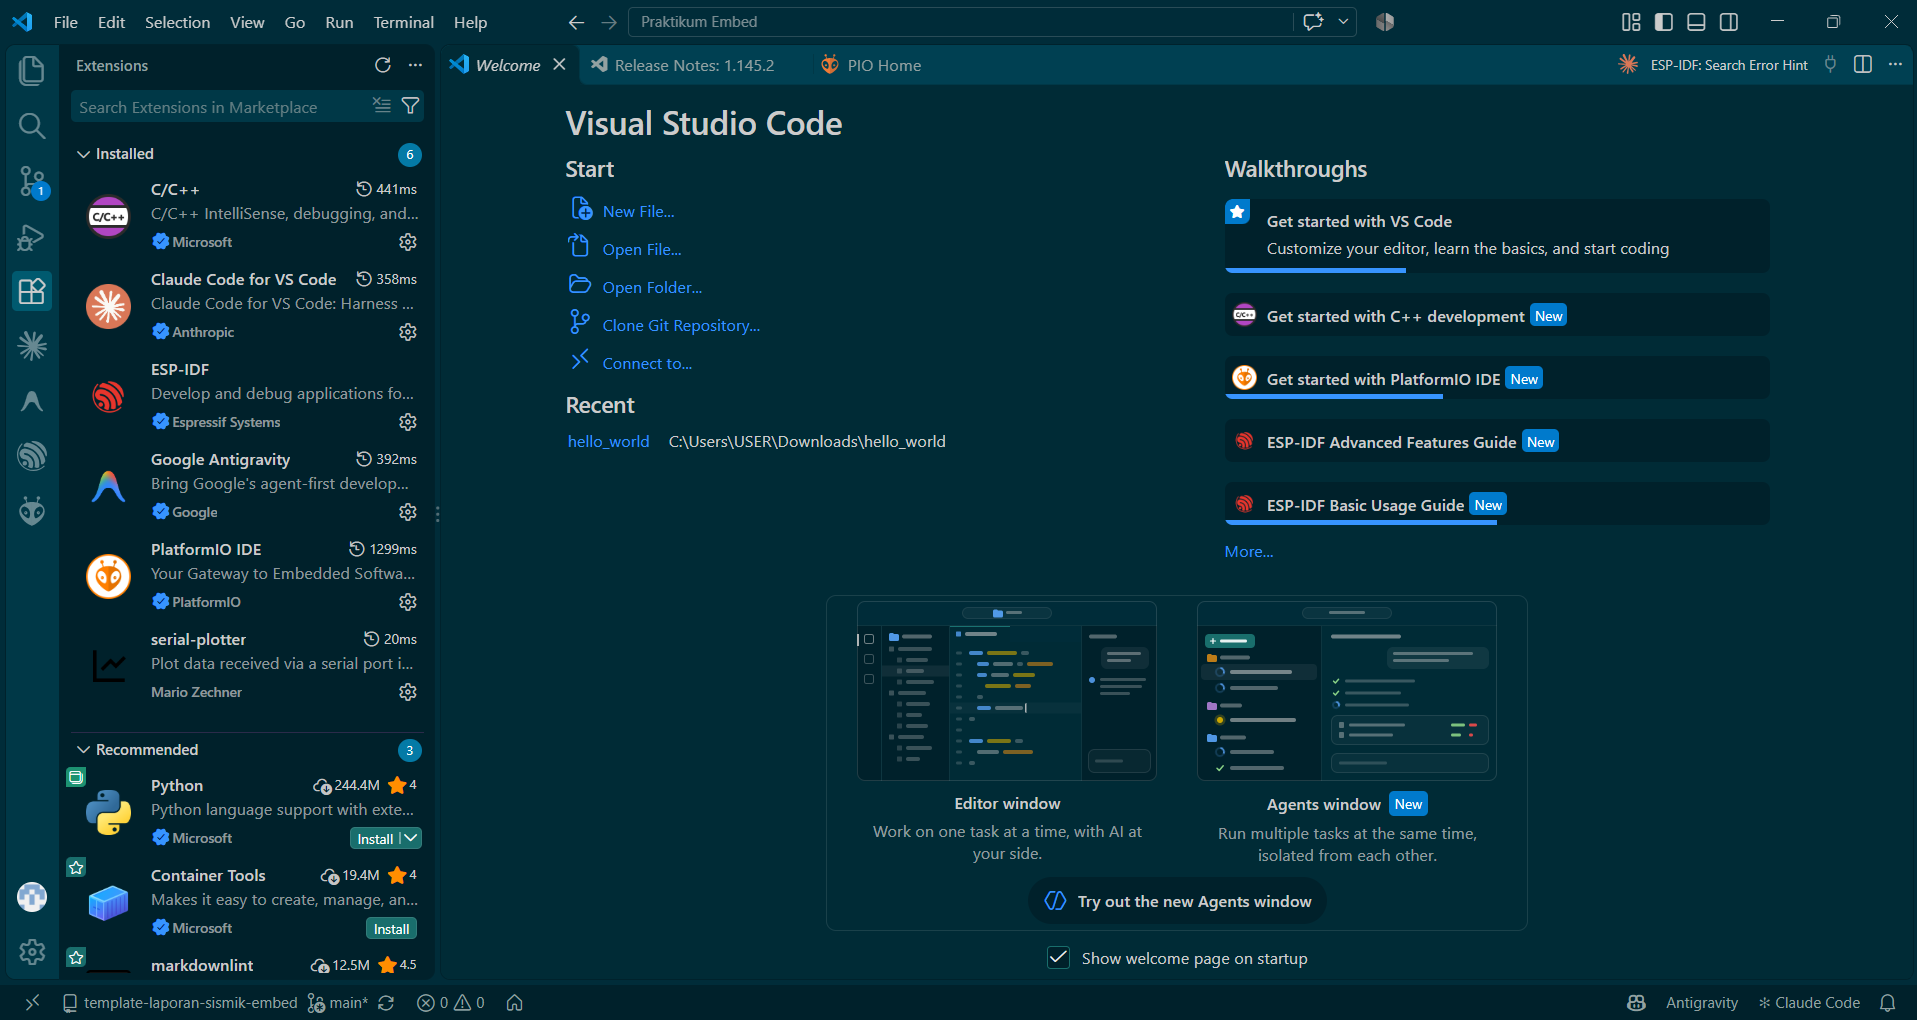
\includegraphics[width=0.9\textwidth]{P1/img/setup_ekstensi.png}%
		}{%
			\fbox{\parbox{0.8\textwidth}{\centering [SCREENSHOT BELUM DITAMBAHKAN: P1/img/setup\_ekstensi.png]}}%
		}
		\caption{Ekstensi PlatformIO IDE dan Serial Plotter terpasang pada VSCode}
		\label{fig:setup-ekstensi}
	\end{figure}

	\begin{figure}[H]
		\centering
		\IfFileExists{P1/img/setup_platform.png}{%
			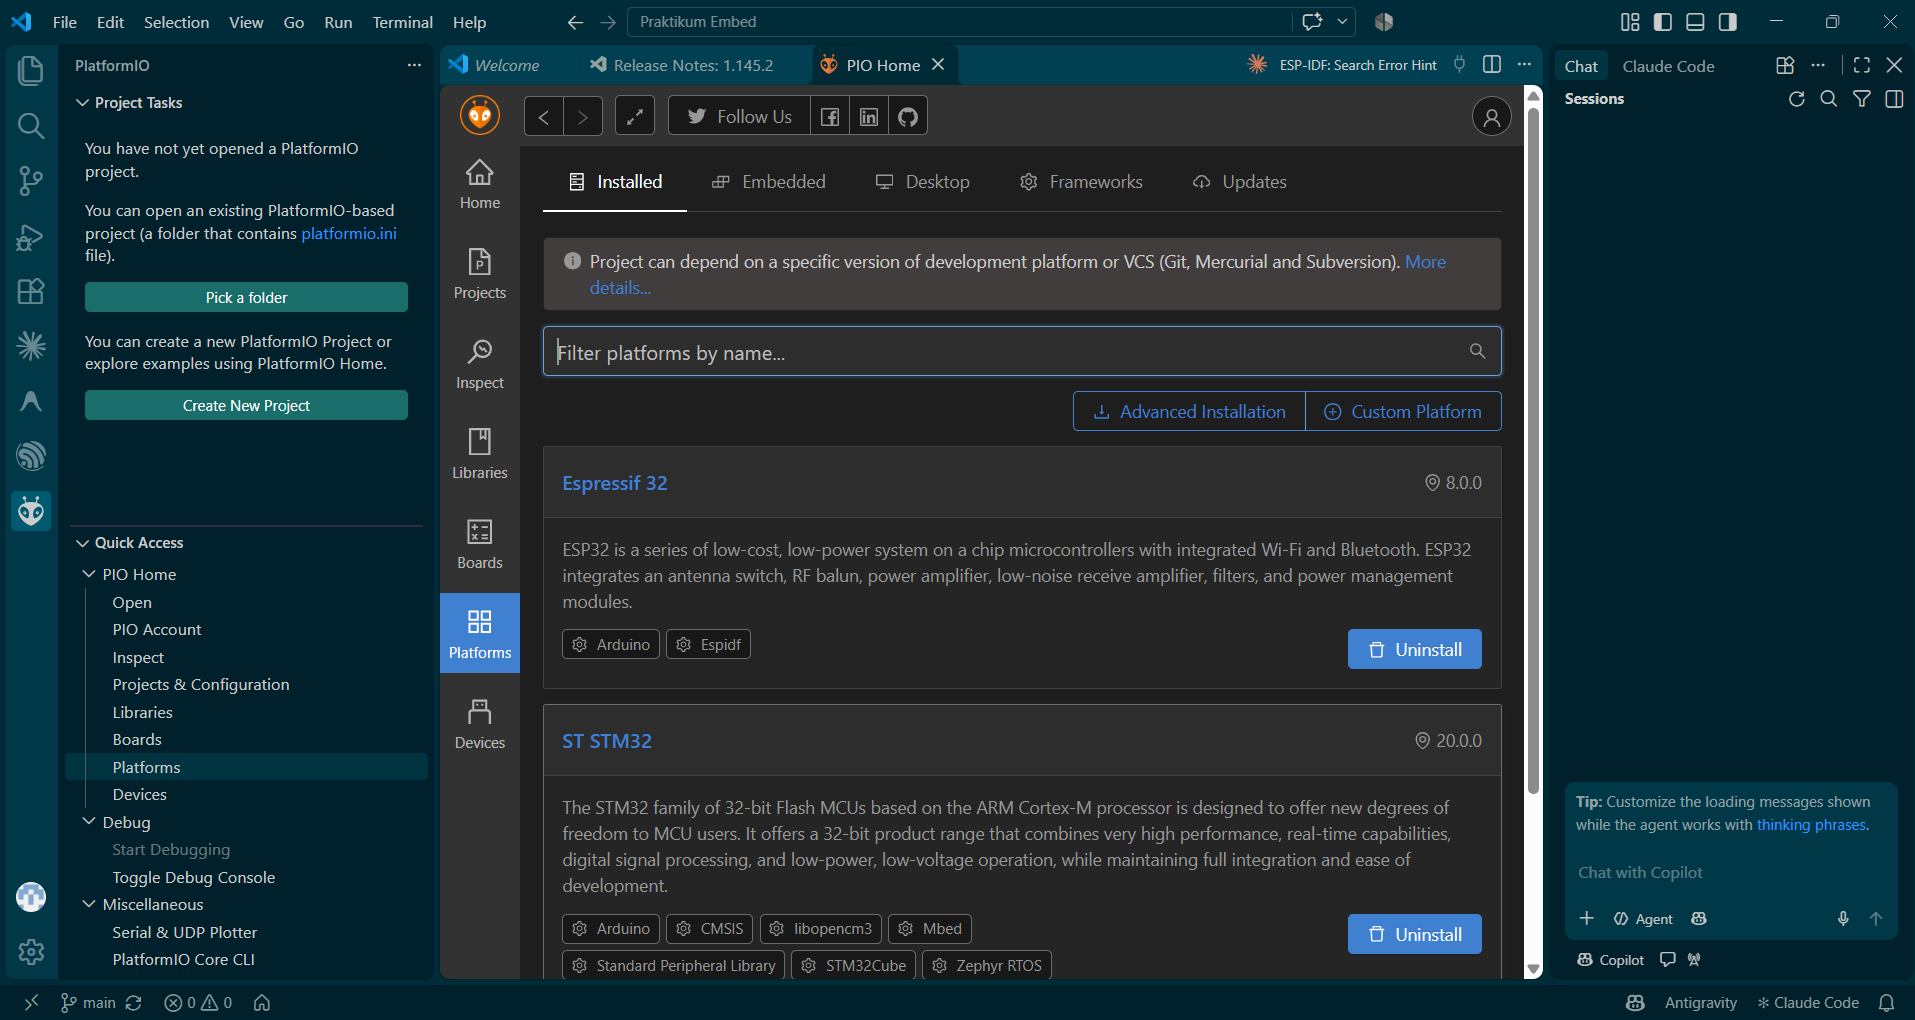
\includegraphics[width=0.9\textwidth]{P1/img/setup_platform.png}%
		}{%
			\fbox{\parbox{0.8\textwidth}{\centering [SCREENSHOT BELUM DITAMBAHKAN: P1/img/setup\_platform.png]}}%
		}
		\caption{Platform Espressif 32 (ESP-IDF) dan ST STM32 terpasang pada PlatformIO}
		\label{fig:setup-platform}
	\end{figure}
\end{enumerate}
